\documentclass{jsarticle}
\usepackage[dvipdfmx]{graphicx}
\begin{document}
In recent years, alongside experimental approaches, simulations utilizing computational tools have been employed to investigate intracellular signaling processes. Simulation research, which seeks to validate hypotheses based on experimental results, is increasingly recognized as a valuable complement to experimental studies. In this paper, we reevaluate the hypothesis that regulatory T cells are involved in the transition from inflammatory microglia to anti-inflammatory microglia from a mathematical modeling (kinetics) standpoint. 
We denote the quantities of inflammatory microglia, anti-inflammatory microglia, and regulatory T cells as M1, M2, and Treg, respectively. Here, we describe the dynamics of M1, M2, and Treg using the following rate equations as the simplest scenario:
\begin{eqnarray}
  \label{eqn:01}
  \frac{dM_{1}(t)}{dt} &=& \alpha f_1(t)- \beta f_2(M_1, T_{reg}) \\
  \label{eqn:02}
  \frac{dM_2(t)}{dt} &=& \beta f_2(M_1, T_{reg}) \\
  \label{eqn:03}
  \frac{dT_{reg}}{dt} &=& f_3(t).
\end{eqnarray}
Equation (\ref{eqn:01}) describes the dynamics of $M_1$. Based on observations that microglia monotonically increase up to a certain limit during sepsis, the function $f_1(t)$ is assumed to be a monotonically increasing function with an upper limit. Additionally, the second term in Equation (\ref{eqn:01}) represents the transition from inflammatory microglia to anti-inflammatory microglia, and it is an increasing function with respect to M1 and Treg. Equation (\ref{eqn:02}) represents the dynamics of $M_2$. It should be noted that (1) + (2) is conserved. Finally, Equation (\ref{eqn:03}) represents the dynamics of Treg. Since it is known that regulatory T cells continue to increase during sepsis, $f_3 > 0$. From the figure, it can be observed that at the onset of sepsis, inflammatory microglia ($M_1$) increase sharply. After a sufficient increase in $M_1$, anti-inflammatory microglia ($M_2$) gradually increase, leading to a decrease in inflammatory microglia cells. The rate of decrease of inflammatory microglia depends strongly on the form of $f_2$ and the parameter $\beta$. To determine these, it is necessary to elucidate the mechanisms of regulatory T cells and anti-inflammatory microglia. Furthermore, by comparing the time series of regulatory T cells and anti-inflammatory microglia quantities, quantitative predictions become feasible.

\begin{figure}[h]
  \centering
    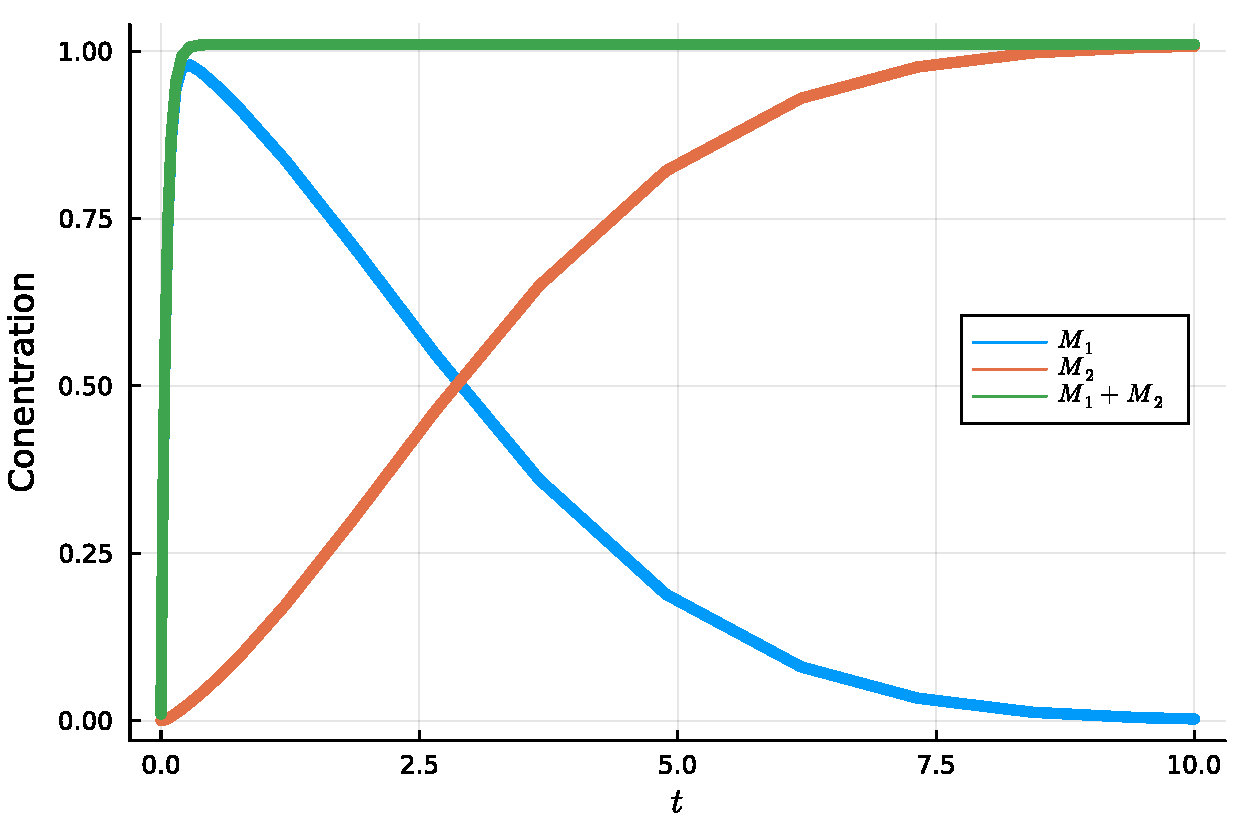
\includegraphics[width=12cm,clip]{../fig/masafig01.pdf}
        \caption{Time series of $M_1$, $M_2$ and $M_1+M_2$. The functional form is $f_1(t):= \gamma\exp{(-\gamma T)}$, $f_2(M_1, T_{reg}):=M_1T_{reg}$,and parameters are $\alpha=$, $\beta=0.1$ and $\gamma=20.0$.}
      \label{fig:01}
  \end{figure}

\end{document}